\documentclass{beamer}
 
\usepackage[utf8]{inputenc}
\usepackage[italian]{babel}
\usepackage[T1]{fontenc}
\usepackage{setspace}

\usepackage{epsfig}
\usepackage{plain}
\usepackage{textcomp}
\usepackage{csquotes}
\usepackage[many]{tcolorbox}
\usepackage{setspace}
\usepackage{amssymb}
\usepackage{color, colortbl}
\usepackage{graphicx}
\usepackage{caption}
\usepackage{subcaption}

\usepackage{booktabs}

\usepackage{array}
\usepackage{makecell}
 
\usetheme{Madrid} 

%Information to be included in the title page:
\titlegraphic{
\includegraphics[width=1.8cm]{unitn.png}
}
\title[Laurea in Informatica]{Identifying and Classifying Symptoms\\within a Patient's Statement}
\author{Nicola Sartorato}
\institute[UNITN]{Universitá di Trento}
\date{23 settembre 2019}

 
\begin{document}

\frame{\titlepage}

\setstretch{1.20}

%\begin{frame}
%\frametitle{Indice}
%
%\begin{itemize}
%\setlength\itemsep{1em}
%\item Il problema e le motivazioni
%\item La soluzione
%\end{itemize}
%
%\end{frame}
 
\begin{frame}
\frametitle{Il macro-obiettivo}

\begin{block}{Il macro-obiettivo}
Sviluppare un agente conversazionale capace di condurre l'\textbf{anamnesi} sostituendosi al medico.
\end{block}

\pause

\begin{alertblock}{L'anamnesi}
È la raccolta dalla voce diretta del paziente di tutte le informazioni utili al medico per effettuare una diagnosi.
\end{alertblock}

\end{frame}

\begin{frame}
\frametitle{Il problema e le motivazioni}
I medici, infatti:

\begin{itemize}
 \item<1-> svolgono il loro lavoro sotto stringenti \textbf{limitazioni di tempo} \pause
 \item<2-> sono occupati principalmente da \textbf{lavori di scrivania }(49.2\% del loro tempo) e solo il 27\% del loro tempo sono a contatto con i pazienti \pause
 \item<3-> l'attività per loro più intensa è l'\textbf{anamnesi}, la quale è:
 \begin{enumerate}

  \item<1-> \textbf{fondamentale}\pause
  \item<2-> ma a volte \textbf{incompleta}
 \end{enumerate}
\end{itemize}

\end{frame}

\begin{frame}
\frametitle{A piccoli passi}

\begin{block}{Il primo ostacolo}
\textbf{Identificare} e \textbf{classificare} i sintomi all'interno di una frase detta da un paziente.
\end{block} \pause

\begin{exampleblock}{Identificare un sintomo}
Individuare all'interno di una frase ogni gruppo di parole adiacenti che, insieme, vogliono dire un sintomo.
\end{exampleblock}\pause

\begin{exampleblock}{Classificare un sintomo}
Mappare i sintomi precedentemente identificati in sintomi specifici che fanno riferimento ad una classificazione.
\end{exampleblock}

\end{frame}

\begin{frame}[c]
\frametitle{}

\begin{center}
\Huge Metodi
\end{center}

\end{frame}

\begin{frame}
\frametitle{Metodi: identificare un sintomo}

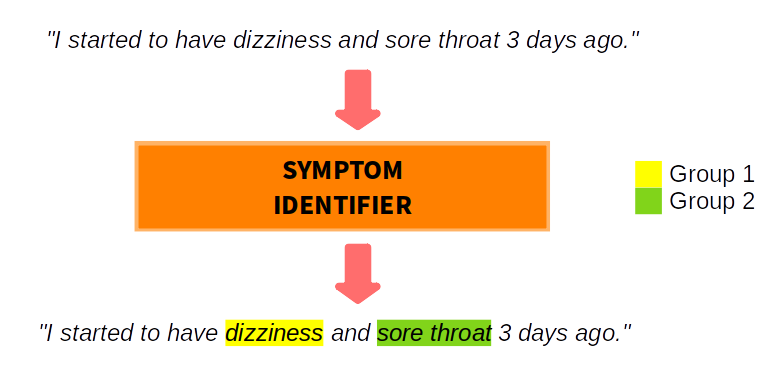
\includegraphics[width=\textwidth]{images/symptom_identifier.png}

Il \textbf{Symptom Identifier} riceve in input la frase del paziente e restituisce i sintomi identificati (i \emph{tokens for predictions}).

\end{frame}

\begin{frame}
\frametitle{Metodi: il Symptom Identifier}
Il \textbf{Symptom Identifier} è composto da tre componenti:\pause
\begin{enumerate}
 \item dal \textbf{Body Part Finder} che evidenzia le parti del corpo all'interno della frase\pause
 \item dal \textbf{Question Answering System } che si occupa di estrarre, usando Machine Reading Comprehension, il problema generico del paziente e quelli delle parti del corpo presenti nella frase. Lo fa sfruttando uno di questi due modelli:\pause
  \begin{itemize}
    \item BERT (Devlin, 2018) \pause
    % è un \emph{pretrained model} che consente di essere \emph{finetuned} su un dataset per Machine Reading Comprehension\pause
    \item R-NET (Wang, 2017) \pause% è un \emph{neural-network model} sviluppato da Microsoft per fare Reading Comprehension
  \end{itemize}
 \item dall'\textbf{Answer Interpreter} che converte le risposte estratte dal QA System in \emph{tokens for predictions}; essi saranno input del Symptom Classifier
\end{enumerate}
\end{frame}

\begin{frame}
\frametitle{Metodi: il Symptom Identifier}
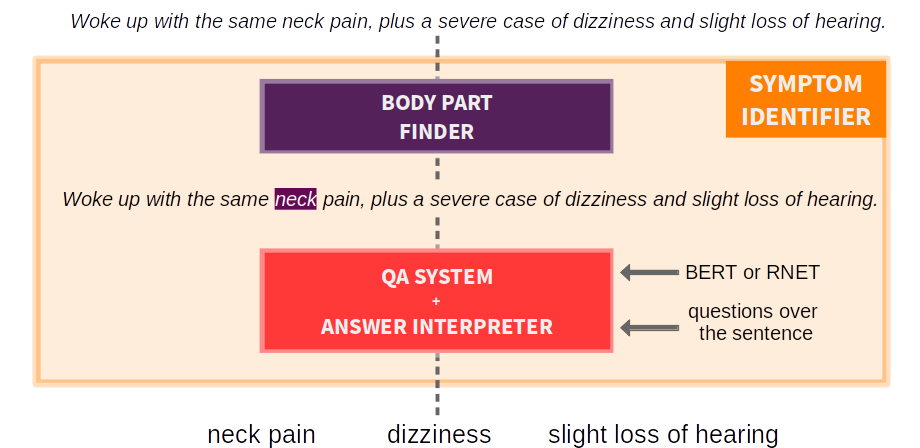
\includegraphics[width=\textwidth]{images/methods_overview1.png}
\end{frame}

\begin{frame}
\frametitle{Metodi: classificare un sintomo}

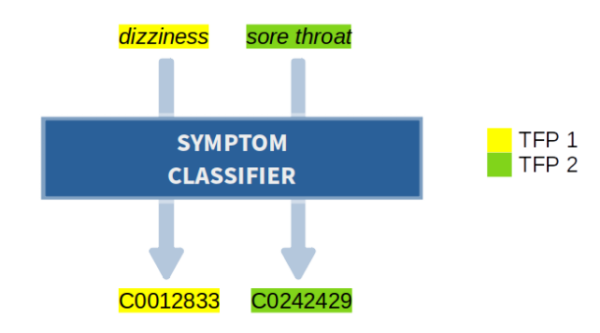
\includegraphics[width=\textwidth]{images/symptom_classifier1.png}

Il \textbf{Symptom Classifier} riceve in input i \emph{tokens for predictions} e restituisce i codici univoci dei sintomi identificati (i CUIs).

\end{frame}

\begin{frame}
\frametitle{La classificazione di sintomi}

La classificazione di sintomi utilizzata è MEDCIN:\pause
\begin{itemize}
  \item si trova all'interno dei dizionari supportati da UMLS (Unified Medical Language System), che fornisce un CUI (Concept Unique Identifier) per ogni suo termine\pause
  \item ha un'organizzazione gerarchica (i.e. ad albero)
\end{itemize}
\end{frame}

\begin{frame}
\frametitle{Metodi: il Symptom Classifier}
Il Symptom Classifier è composto da due componenti:\pause
\begin{enumerate}
  \item il \textbf{Vectorifier}, che ha il compito di vettorizzare i tokens for predictions in due possibili tipi di embeddings:\pause
    \begin{enumerate}
      \item GloVe embeddings (Pennington, 2014)\pause
      \item BERT embeddings (Devlin, 2018)\pause
    \end{enumerate}
  \item il \textbf{Symptom Tree Mapper}, il cui scopo è ritornare, dato un \emph{token for prediction}, il CUI del sintomo predetto. Ogni sintomo appartenente all'albero ha un suo rappresentante (la media dei vettori delle parole nel nome del sintomo).
  \pause
\begin{alertblock}{Criterio di predizione}    
Viene calcolata la cosine similarity tra ogni \emph{token for prediction} vettorizzato e il rappresentante di ogni sintomo appartenente all'albero. Il sintomo con maggiore similarità verrà predetto.
\end{alertblock}
\end{enumerate}
\end{frame}

\begin{frame}
\frametitle{Metodi: il Symptom Classifier}
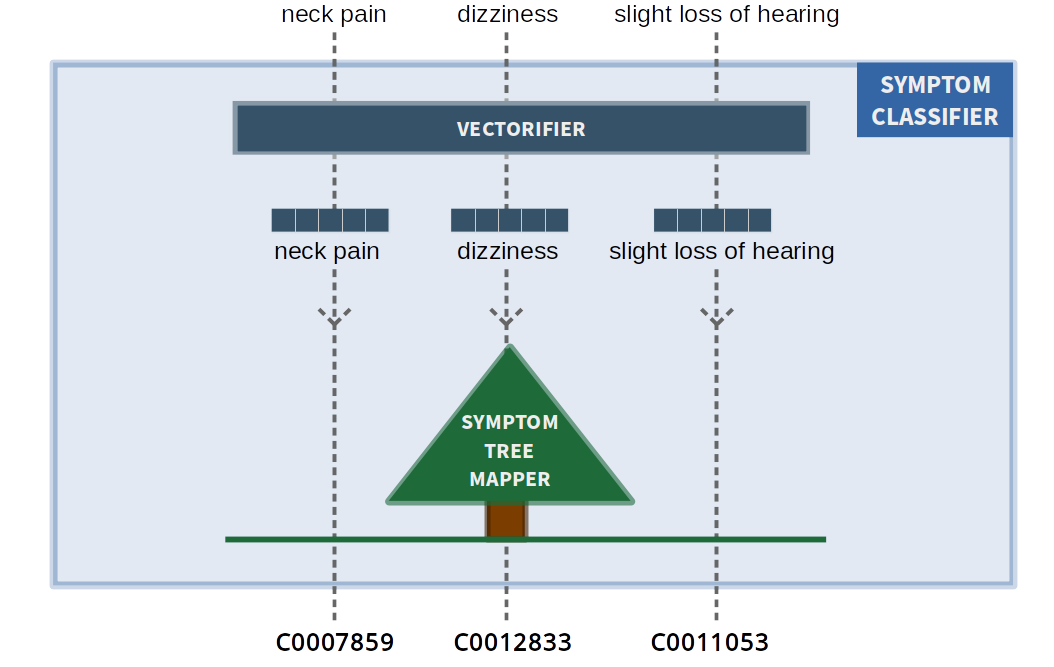
\includegraphics[width=\textwidth]{images/methods_overview2.png}
\end{frame}

\begin{frame}
\frametitle{Il dataset}
Al momento, non ci sono dataset utilizzabili per la classificazione di sintomi. Si è rivelato necessario:
\begin{itemize}
  \item estrarre 336 frasi dai post di un forum medico (doctorslounge.com)
  \item taggare i sintomi presenti nelle frasi
\end{itemize}
\end{frame}
\begin{frame}[c]
\frametitle{}
\begin{center}
\Huge Risultati
\end{center}
\end{frame}

\begin{frame}
\frametitle{Risultati: valutare il Symptom Identifier}
Per valutare il Symptom Identifier i \emph{tokens for predictions} sono stati classificati in:\pause
\begin{enumerate}
  \item \texttt{correct} tokens\pause
  \item \texttt{redundant} tokens\pause
  \item \texttt{non-sense} tokens\pause
  \item \texttt{wrong} tokens
\end{enumerate}
\end{frame}

\definecolor{green}{rgb}{0.8,0.9,0.8}
\definecolor{lightgreen}{rgb}{0.89, 0.94, 0.89}
\definecolor{red}{rgb}{1,0.89,0.89}

\begin{frame}
\frametitle{Risultati: valutare il Symptom Identifier}

\begin{equation}
score = \texttt{\#correct} - \texttt{\#non sense} - \texttt{\#wrong} - \texttt{\#missing}
\label{score}
\end{equation}

\begin{center}
  \begin{table}[h]
  \centering
     \begin{tabular}{| c | c | c | c |} 
     \hline
     \# of & BERT & R-NET \\ [0.5ex] 
     \hline\hline
     \rowcolor{green}
     \texttt{correct} & 423 & 427 \\ 
     \hline
     \rowcolor{lightgreen}
     \texttt{redundant} & 275 & 195 \\
     \hline
     \rowcolor{red}
     \texttt{non sense} & 122 & 247 \\
     \hline
     \rowcolor{red}
     \texttt{wrong} & 8 & 14 \\
     \hline
     \rowcolor{red}
     \texttt{missing} & 61 & 74 \\
     \hline
     \textbf{score} & \textbf{232} & \textbf{92} \\ 
     \hline
    \end{tabular}
    \caption{Confronto dello score tra BERT e R-NET come calcolato in (\ref{score}).}
 \end{table}
\end{center}
\end{frame}

\begin{frame}
\frametitle{Risultati: valutare il Symptom Classifier}
Per valutare il Symptom Classifier le predizioni sono state divise in:
\pause\begin{itemize}
  \item \texttt{correct}, se la predizione si trova in uno dei sottoalberi di un sintomo presente nella frase; a loro volta divise in:\pause
    \begin{itemize}
      \item \texttt{non-redundant}, se il sottoalbero in questione non è stato marcato come già associato\pause
      \item \texttt{redundant}, se invece è già stato marcato come  associato\pause
    \end{itemize}
  \item \texttt{wrong}, se la predizione non si trova in nessun sottoalbero
\end{itemize}
\end{frame}

\begin{frame}
\frametitle{Risultati: valutare il Symptom Classifier}
Assieme al Symptom Classifier sono state valutate le seguenti opzioni:\pause
\begin{itemize}
  \item diversi tipi di embeddings \pause
  \item se usare o meno il Body Part Finder \pause
  \item se cercare o meno il sintomo solo nei sottoalberi relativi alle parti del corpo trovate nella frase (l'opzione ``pruning'') \pause
  \item diversi \emph{minimum similarity thresholds}: il valore minimo di similarità affinché una predizione sia ritenuta valida
\end{itemize}
\end{frame}

\begin{frame}
\frametitle{Risultati: valutare il Symptom Classifier}
\begin{center}
 \begin{table}[h]
 \centering
   \begin{tabular}{| c | c | c | c | c |} 
   \hline
   \thead{\texttt{embedding}\\\texttt{type}} & \thead{\texttt{accuracy}} & \thead{\texttt{correct}\\\texttt{predictions}} & \thead{\texttt{harmonic}\\\texttt{mean}} & \thead{\texttt{missed}\\\texttt{symptoms}} \\ [0.5ex] 
   \hline\hline
   \texttt{GloVe 50} & 55.5 \% & 40.1 \% & 46.5 \% & 208 \\ 
   \hline
   \texttt{GloVe 100} & 55.2 \% & 39.1 \% & 45.8 \% & 209 \\
   \hline
   \rowcolor{green}
   \texttt{GloVe 200} & 59.1 \% & 43.7 \% & 50.2 \% & 191 \\
   \hline
   \rowcolor{green}
   \texttt{GloVe 300} & 59.3 \% & 42.2 \% & 49.3 \% & 190 \\
   \hline
   \texttt{BERT emb.} & 46.7 \% & 32.9 \% & 38.6 \% & 249 \\
   \hline
  \end{tabular}
 \caption{Confronto tra diversi tipi di embeddings usando indici diversi. La media armonica tra \texttt{accuracy} e \texttt{correct predictions} indica che GloVe 200 e GloVe 300 hanno performance migliori degli altri tipi.}
 \end{table}
\end{center}
\end{frame}

\begin{frame}
\frametitle{Risultati: valutare il Symptom Classifier}
\begin{figure}
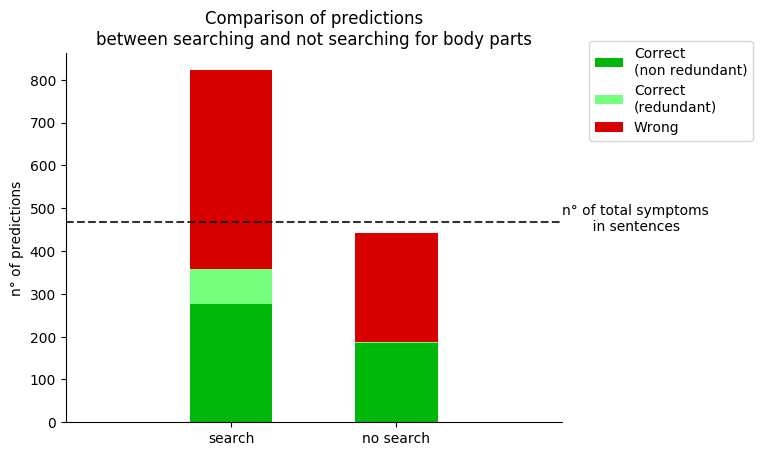
\includegraphics[width=10cm]{images/graphs/comparison_search_bp}
    \caption{Confronto della composizione delle predizioni quando il Body Part Finder è attivo (\texttt{search}) e quando non lo è (\texttt{no search}).}
\end{figure}
\end{frame}

\begin{frame}
\frametitle{Risultati: valutare il Symptom Classifier}
\begin{center}
 \begin{table}[h]
 \centering
   \begin{tabular}{| c | c | c | c |} 
   \hline
    & \thead{\texttt{accuracy}} & \thead{\texttt{correct}\\\texttt{predictions}} &  \thead{\texttt{missed}\\\texttt{symptoms}} \\ [0.5ex] 
   \hline\hline
   \texttt{pruning} & 59.1 \% & 43.7 \% & 191 \\
   \hline
   \texttt{no pruning} & 43.7 \% & 36.0 \% & 263 \\
   \hline
  \end{tabular}
 \caption{Confronto fra indici quando l'opzione ``pruning'' è attiva (\texttt{pruning}) e quando non lo è (\texttt{no pruning}). L'introduzione di questa opzione provoca un miglioramento del $15.4\%$ nell'accuracy e del $7.7\%$ nelle predizioni corrette.}
 \end{table}
\end{center}
\end{frame}

\begin{frame}
\frametitle{Risultati: valutare il Symptom Classifier}
\begin{figure}
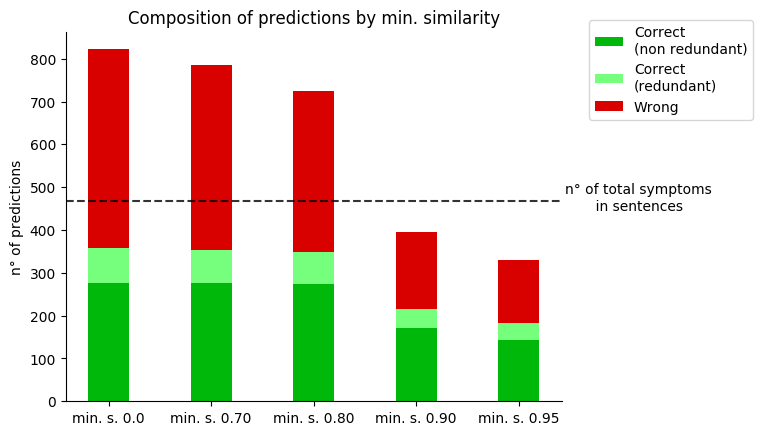
\includegraphics[width=10.5cm]{images/graphs/comparison_min_similarity.png}
    \caption{Confronto della composizione delle predizioni usando diversi \textit{minimum similarity thresholds} ($0.00$, $0.70$, $0.80$, $0.90$, $0.95$).}
\end{figure}
\end{frame}

%\begin{frame}
%\frametitle{Risultati: valutare il Symptom Classifier}
%\begin{center}
% \begin{table}[h]
% \centering
%   \begin{tabular}{| c | c | c | c | c |} 
%   \hline
%    \thead{\texttt{minimum}\\\texttt{similarity}} & \thead{\texttt{accuracy}} & \thead{\texttt{correct}\\\texttt{predictions}} & \thead{\texttt{medium}\\\texttt{attempts}} & \thead{\texttt{missed}\\\texttt{symptoms}} \\ [0.5ex] 
%   \hline\hline
%   \texttt{0.00} & 59.1 \% & 43.7 \% & 1.8 & 191 \\ 
%   \hline
%   \texttt{0.70} & 59.1 \% & 45.1 \% & 1.7 & 191 \\
%   \hline
%   \rowcolor{green}
%   \texttt{0.80} & 58.7 \% & 48.0 \% & 1.5 & 193 \\
%   \hline
%   \texttt{0.90} & 36.8 \% & 54.7 \% & 0.8 & 295 \\
%   \hline
%   \texttt{0.95} & 30.6 \% & 55.3 \% & 0.7 & 324 \\
%   \hline
%  \end{tabular}
% \caption{\label{tab:minsim}Confronto fra indici usando diversi \textit{minimum similarity thresholds}.}
% \end{table}
%\end{center}
%\end{frame}

\begin{frame}
\frametitle{Conclusioni}
\begin{itemize}
\item I risultati sono complessivamente positivi perché, anche usando usando una rappresentazione semplificata, il modello raggiunge: 
 \begin{itemize}
  \item il 58.7\% di accuracy
  \item il 48.0\% di predizioni corrette
  \item facendo 1.5 \texttt{medium attempts}
 \end{itemize}\pause
 \item Il fatto che i risultati dipendano molto dalle rappresentazioni dei sintomi indica che c'è molto margine di miglioramento.\pause
 \item Il Symptom Classifier è la prima componente da migliorare: infatti, si passa dall'84.8\% di \emph{tokens for predictions} corretti al 48.0\% di previsioni corrette.
\end{itemize}
\end{frame}

\begin{frame}
\frametitle{Conclusioni: future work}
Questa componente può essere usata come base per una futura che riesca a focalizzare le domande su sintomi correlati a quelli già scoperti:
  \begin{itemize}\pause
  \item usare \texttt{cui2vec} (Beam, 2018) come rappresentazioni per i sintomi e algoritmi di clustering per esplorare gruppi di sintomi correlati
\end{itemize}
\end{frame}

\begin{frame}[plain, c]
\frametitle{}
\begin{center}
\Huge \emph{Grazie per l'attenzione}
\end{center}
\end{frame}

\end{document}
